\documentclass[11pt]{article}
\usepackage{latexsym,amsmath,amsfonts,amssymb,mathrsfs}
\usepackage[latin1]{inputenc}
\usepackage{tikz}
\usetikzlibrary{decorations.pathreplacing}
\usetikzlibrary{shapes}
\usepackage{tikz}
\usetikzlibrary{calc}
\usetikzlibrary{decorations.text}
\usetikzlibrary{shapes}
\usetikzlibrary{decorations.pathmorphing}
\usetikzlibrary{decorations.pathreplacing}
\usetikzlibrary{arrows.meta}
\tikzset{%%
  >={To[length=5pt]}
  }
\usetikzlibrary{shapes, shapes.geometric, shapes.symbols, shapes.arrows, shapes.multipart, shapes.callouts, shapes.misc}
\tikzset{snake it/.style={decorate, decoration=snake}}
\tikzset{7brane/.style={circle, draw=black, fill=black,ultra thick,inner sep=1.5 pt, minimum size=1 pt,}, c/.default={4pt}}
\tikzset{cross/.style={cross out, draw=black,thick, minimum size=2*(#1-\pgflinewidth), inner sep=0pt, outer sep=0pt}, cross/.default={5pt}}
\tikzset{big7brane/.style={circle, draw=black, fill=black,ultra thick,inner sep=2.5 pt, minimum size=1 pt,}, c/.default={4pt}}
\tikzset{u/.style={circle, draw=black, fill=white,inner sep=2 pt, minimum size=2 pt,},f/.style={square, draw=black, fill=white,ultra thick,inner sep=4 pt, minimum size=2 pt,}}
\tikzset{so/.style={circle, draw=black, fill=red,inner sep=2 pt, minimum size=2 pt,},f/.style={square, draw=black, fill=white,ultra thick,inner sep=4 pt, minimum size=2 pt,}}
\tikzset{sp/.style={circle, draw=black, fill=blue,inner sep=2 pt, minimum size=2 pt,},f/.style={square, draw=black, fill=white,ultra thick,inner sep=4 pt, minimum size=2 pt,}}
\tikzset{uf/.style={rectangle, draw=black, fill=white,inner sep=3 pt, minimum size=4 pt,}}
\tikzset{spf/.style={rectangle, draw=black, fill=blue, thick,inner sep=3 pt, minimum size=4 pt, circle, draw=black, fill=blue,thick,inner sep=2 pt, minimum size=2 pt,},f/.style={square, draw=black, fill=white,ultra thick,inner sep=4 pt, minimum size=2 pt,}}
\tikzset{sof/.style={rectangle, draw=black, fill=red, thick,inner sep=3 pt, minimum size=4 pt,}}
\usetikzlibrary{positioning}
\usetikzlibrary{arrows}
\usetikzlibrary{decorations.pathreplacing}
\usetikzlibrary{shapes}

\begin{document}

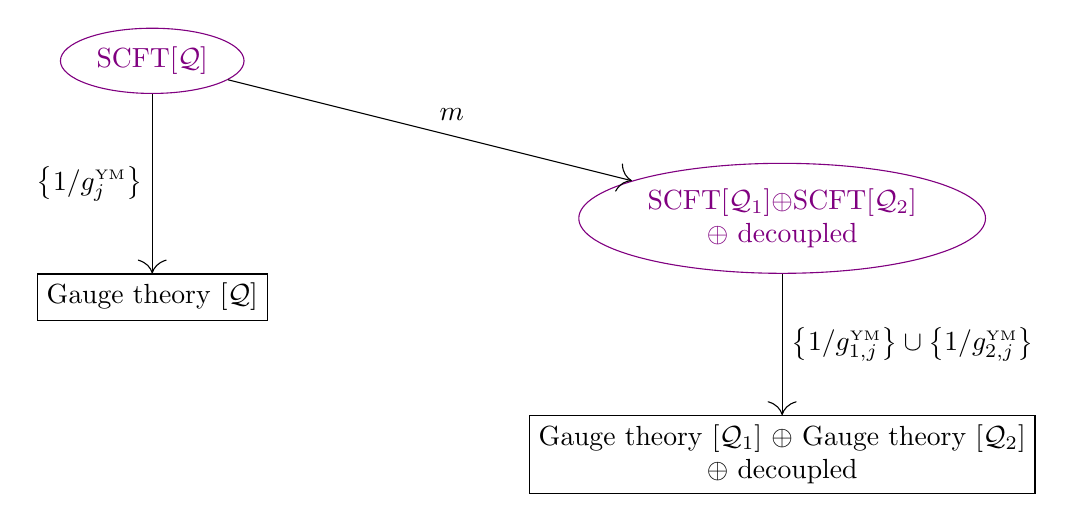
\begin{tikzpicture}
\node[draw,ellipse,violet] (cft1) at (0,4) {SCFT$[\mathcal{Q}]$};
\node[draw,ellipse,violet,align=center] (cft2) at (8,2) {SCFT$[\mathcal{Q}_1] \oplus $SCFT$[\mathcal{Q}_2]$\\ $\oplus$ decoupled};
\path[->,black] (cft1) edge node[anchor=south west] {$m$} (cft2);

\node[draw,rectangle] (g1) at (0,1) {Gauge theory $[\mathcal{Q}]$};
\node[draw,rectangle,align=center] (g2) at (8,-1) {Gauge theory $[\mathcal{Q}_1]$ $\oplus$ Gauge theory $[\mathcal{Q}_2]$\\ $\oplus$ decoupled};
\path[->,black] (cft1) edge node[anchor=east] {$\left\{ 1/g_{j}^{\text{\tiny YM}} \right\}$} (g1);
\path[->,black] (cft2) edge node[anchor=west] {$\left\{ 1/g_{1,j}^{\text{\tiny YM}} \right\} \cup \left\{ 1/g_{2,j}^{\text{\tiny YM}} \right\}  $} (g2);

\end{tikzpicture}

\end{document}